\documentclass{../cssheet}

%--------------------------------------------------------------------------------------------------------------
% Basic meta data
%--------------------------------------------------------------------------------------------------------------

\title{Kongruenzabbildungen}
\author{Prof. Dr. Christian Spannagel}
\date{\today}
\hypersetup{%
    pdfauthor={\theauthor},%
    pdftitle={\thetitle},%
    pdfsubject={Aufgabenblatt Geometrie},%
    pdfkeywords={geometrie}
}


%--------------------------------------------------------------------------------------------------------------
% document
%--------------------------------------------------------------------------------------------------------------

\begin{document}
\printtitle

\textbf{Aufgabe 1 (Kongruenzabbildungen):}  Untersucht die verschiedenen Kongruenzabbildungen auf ihre Eigenschaften und füllt die Tabelle aus. Überprüft anhand geeigneter Beispiele. Welche Eigenschaften haben alle Kongruenzabbildungen? (Also: Was macht eine Kongruenzabbildung aus?)

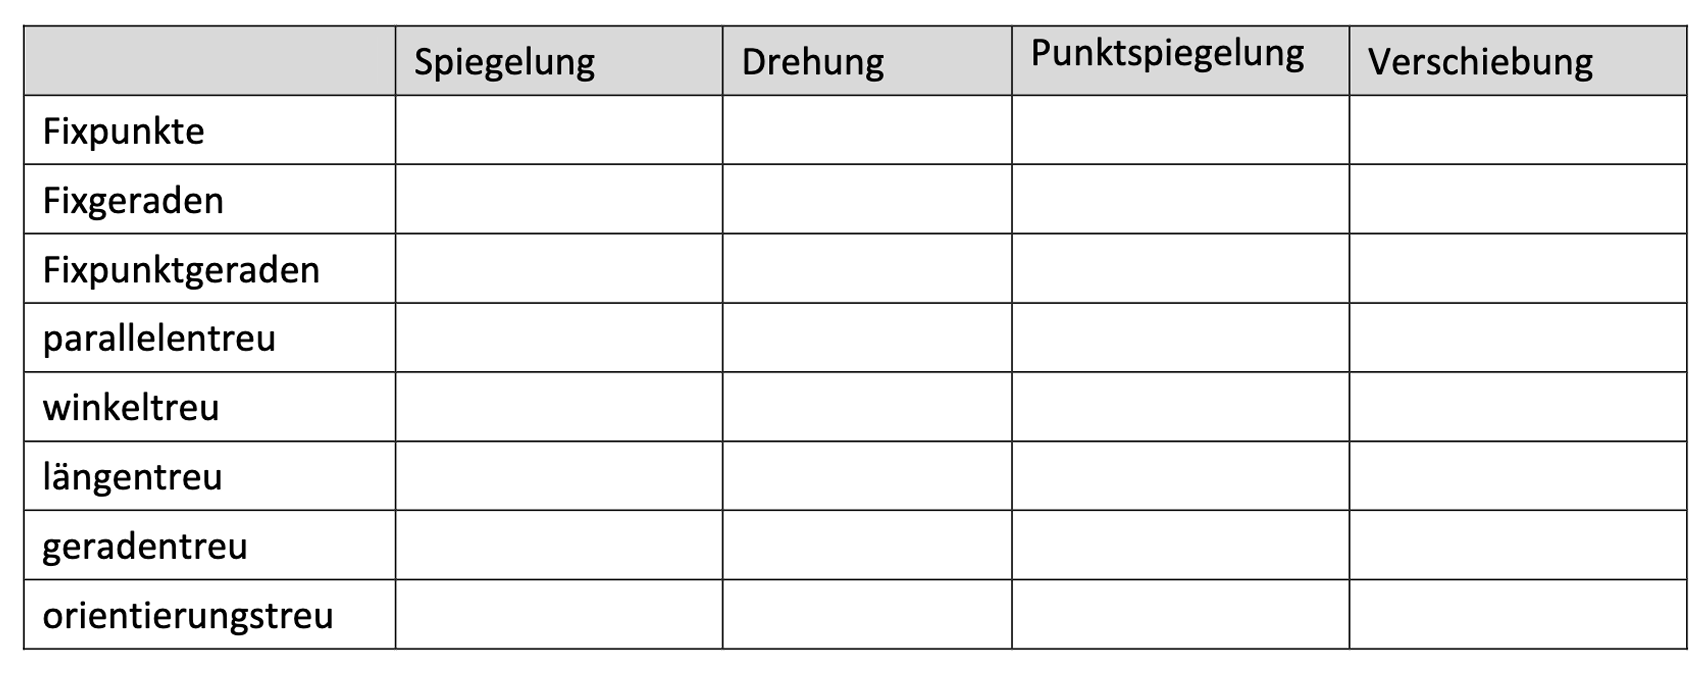
\includegraphics[width=16cm]{tabelle.png}
\vspace*{10mm}

\printlicense

\printsocials

\end{document}
